\documentclass[tikz,border=4pt]{standalone}
\usepackage[T1]{fontenc}
\usepackage{lmodern}
\renewcommand{\familydefault}{\sfdefault}
\usetikzlibrary{shapes.geometric,positioning,arrows.meta,calc}
\tikzset{
  node distance=6mm,
  every node/.style={font=\footnotesize,align=center,execute at begin node={\hyphenpenalty=10000\relax}},
  base/.style={draw=gray!60,fill=gray!12,minimum height=7mm,inner sep=2pt},
  term/.style={base,rounded corners=3.5mm,text width=30mm},
  proc/.style={base,text width=32mm},
  err/.style={base,text width=30mm,fill=gray!22},
  io/.style={base,trapezium,trapezium left angle=72,trapezium right angle=108,trapezium stretches=true,text width=28mm},
  dec/.style={base,diamond,aspect=2.4,text width=27mm,inner sep=0pt},
  go/.style={-{Stealth[length=2mm]},draw=gray!55!black},
  lab/.style={font=\scriptsize,fill=white,inner sep=1pt},
}

\begin{document}
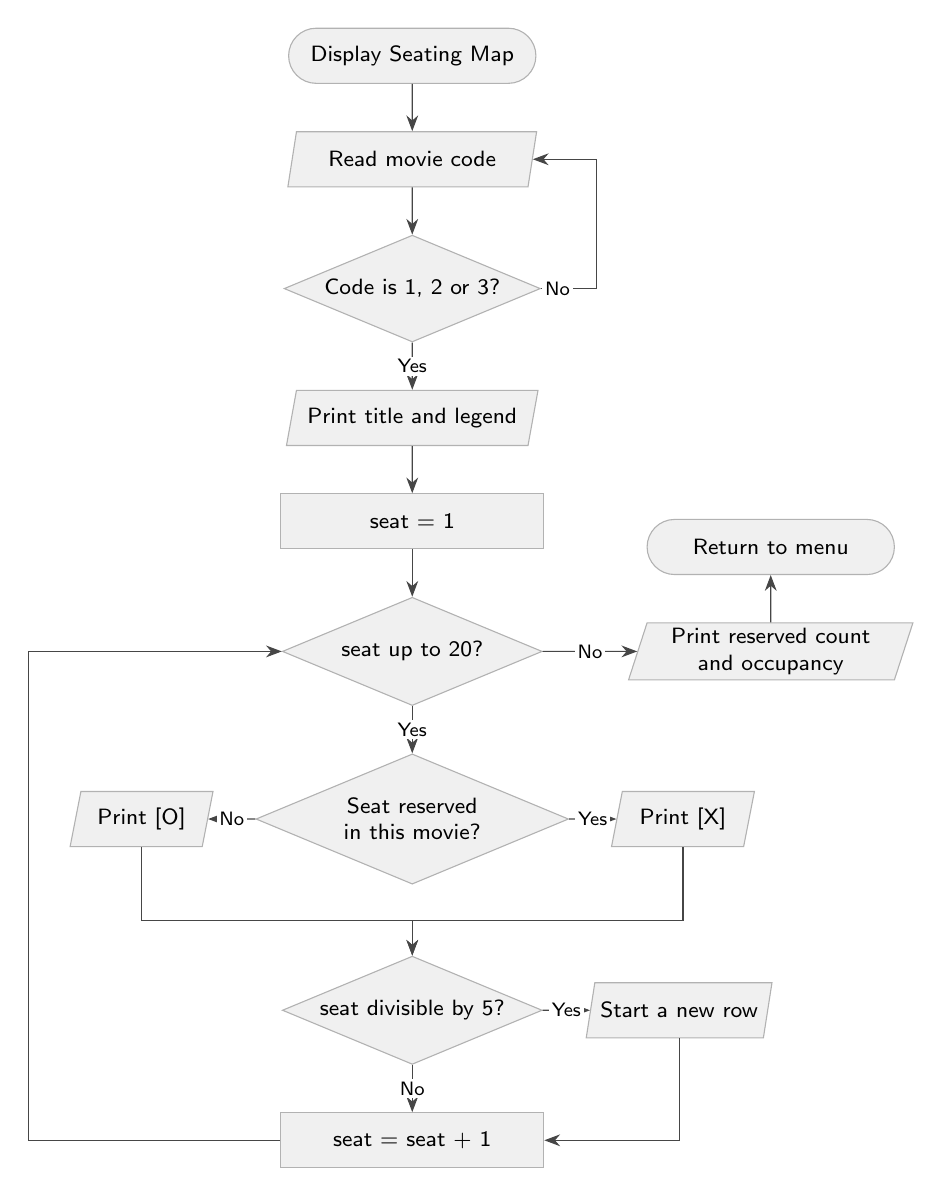
\begin{tikzpicture}
\node[term] (s) {Display Seating Map};
\node[io,below=of s] (r) {Read movie code};
\node[dec,below=of r] (c) {Code is 1, 2 or 3?};
\node[io,below=of c] (h) {Print title and legend};
\node[proc,below=of h] (i) {seat = 1};
\node[dec,below=of i] (d) {seat up to 20?};
\node[dec,below=of d] (q) {Seat reserved in this movie?};
\node[io,right=6mm of q,text width=14mm] (x) {Print [X]};
\node[io,left=6mm of q,text width=14mm] (o) {Print [O]};
\node[dec,below=9mm of q] (f) {seat divisible by 5?};
\node[io,right=6mm of f,text width=20mm] (l) {Start a new row};
\node[proc,below=of f] (n) {seat = seat + 1};
\node[io,right=12mm of d,text width=30mm] (p) {Print reserved count and occupancy};
\node[term,above=of p] (e) {Return to menu};
\draw[go] (s)--(r);\draw[go] (r)--(c);
\draw[go] (c)--node[lab]{Yes}(h);
\draw[go] (c.east)--node[lab,pos=.3]{No}++(7mm,0)|-(r.east);
\draw[go] (h)--(i);\draw[go] (i)--(d);
\draw[go] (d)--node[lab]{Yes}(q);
\draw[go] (d)--node[lab]{No}(p);
\draw[go] (p)--(e);
\draw[go] (q)--node[lab]{Yes}(x);
\draw[go] (q)--node[lab]{No}(o);
\draw[go] (x.south)|-($(f.north)+(0,4.5mm)$)--(f.north);
\draw[go] (o.south)|-($(f.north)+(0,4.5mm)$)--(f.north);
\draw[go] (f)--node[lab]{Yes}(l);
\draw[go] (f)--node[lab]{No}(n);
\draw[go] (l.south)|-(n.east);
\draw[go] (n.west)--++(-32mm,0)|-(d.west);
\end{tikzpicture}
\end{document}
